\documentclass[a0,portrait]{a0poster}

\usepackage{multicol}
\columnsep=100pt
\columnseprule=3pt

\usepackage{ragged2e}
\usepackage[utf8]{inputenc}		% Codificacao do documento (conversão automática dos acentos)
\usepackage{times}
\usepackage{graphicx}
\graphicspath{{../}}
\usepackage{booktabs}
\usepackage[font=small,labelfont=bf]{caption}
\usepackage{amsfonts, amsmath, amsthm, amssymb, marvosym}
\usepackage{wrapfig}
\usepackage{enumitem}
\usepackage{fancyvrb}
\usepackage{xspace}
\usepackage[svgnames,usenames,dvipsnames]{xcolor}

\usepackage{listings}
\usepackage{listingsutf8}

\lstset{literate=
	{ã}{{\~a}}1 {ẽ}{{\~e}}1 {ĩ}{{\~i}}1 {õ}{{\~o}}1 {ũ}{{\~u}}1
	{Ã}{{\~A}}1 {Ẽ}{{\~E}}1 {Ĩ}{{\~I}}1 {Õ}{{\~O}}1 {Ũ}{{\~U}}1	
	{á}{{\'a}}1 {é}{{\'e}}1 {í}{{\'i}}1 {ó}{{\'o}}1 {ú}{{\'u}}1
	{Á}{{\'A}}1 {É}{{\'E}}1 {Í}{{\'I}}1 {Ó}{{\'O}}1 {Ú}{{\'U}}1
	{à}{{\`a}}1 {è}{{\`e}}1 {ì}{{\`i}}1 {ò}{{\`o}}1 {ù}{{\`u}}1
	{À}{{\`A}}1 {È}{{\'E}}1 {Ì}{{\`I}}1 {Ò}{{\`O}}1 {Ù}{{\`U}}1
	{ä}{{\"a}}1 {ë}{{\"e}}1 {ï}{{\"i}}1 {ö}{{\"o}}1 {ü}{{\"u}}1
	{Ä}{{\"A}}1 {Ë}{{\"E}}1 {Ï}{{\"I}}1 {Ö}{{\"O}}1 {Ü}{{\"U}}1
	{â}{{\^a}}1 {ê}{{\^e}}1 {î}{{\^i}}1 {ô}{{\^o}}1 {û}{{\^u}}1
	{Â}{{\^A}}1 {Ê}{{\^E}}1 {Î}{{\^I}}1 {Ô}{{\^O}}1 {Û}{{\^U}}1
	{œ}{{\oe}}1 {Œ}{{\OE}}1 {æ}{{\ae}}1 {Æ}{{\AE}}1 {ß}{{\ss}}1
	{ű}{{\H{u}}}1 {Ű}{{\H{U}}}1 {ő}{{\H{o}}}1 {Ő}{{\H{O}}}1
	{ç}{{\c c}}1 {Ç}{{\c C}}1 {ø}{{\o}}1 {å}{{\r a}}1 {Å}{{\r A}}1
	{€}{{\EUR}}1 {£}{{\pounds}}1
}

\lstdefinestyle{codeStyle}{
	commentstyle=\color{black},
	basicstyle=\ttfamily\footnotesize,
	breakatwhitespace=false,         
	breaklines=true,                 
	captionpos=b,                    
	keepspaces=true,                 
	numbers=left,                    
	numbersep=5pt,                  
	showspaces=false,                
	showstringspaces=false,
	showtabs=false,                  
	tabsize=2
}
\renewcommand{\lstlistingname}{Código}
\renewcommand{\tablename}{Tabela}
\renewcommand{\figurename}{Figura}
\newcommand\itemadjust{\itemsep.5em \parskip0pt \parsep0pt}

% ---
% Formatação de código-fonte
% ---
\usepackage{listings}
\usepackage{algpseudocode}




\begin{document}
%---------------------------------------------------------------
%	POSTER HEADER 
%---------------------------------------------------------------
\begin{minipage}[c]{\linewidth}
	\vspace{0.1cm}
	\noindent\makebox[\textwidth][c]{
		
	\begin{minipage}[c]{0.15\linewidth}
		\begin{center}
			
\includegraphics[width=9cm]{fig/logoPUCRS.pdf}
		\end{center}
	\end{minipage}
	
	\begin{minipage}[c]{0.70\linewidth}
		\centering
		\veryHuge \color{NavyBlue} 
		\textbf{Adversarial Hierarchical-Task Network para Jogos em Tempo Real}\\
		
		\color{Black}
		\huge \textbf{Matheus de Souza Redecker}\\
		\Large \textbf{Orientador: Prof. Felipe Rech Meneguzzi}\\
		Curso de Ciência da Computação --
		Pontifícia Universidade Católica do Rio Grande do Sul\\
		\Large \Letter ~ \texttt{matheus.redecker@acad.pucrs.br}\\
	\end{minipage}
	
	\begin{minipage}[c]{0.15\linewidth}
		\begin{center}
			
\includegraphics[width=9cm]{fig/logoFacin.pdf}
		\end{center}
	\end{minipage}}
	\\[0.1cm]%
% A bit of extra whitespace between the header and poster content
\end{minipage}

\vspace{1cm}

%---------------------------------------------------------------

\begin{multicols}{2} 
	%---------------------------------------------------------------
	%	ABSTRACT
	%---------------------------------------------------------------
	\color{NavyBlue}
	\color{Black}
	\raggedright
	\Large
	%---------------------------------------------------------------
	%	Motivação
	%---------------------------------------------------------------
	\color{NavyBlue}
	\section*{\huge Motiva\c{c}\~ao}
	\color{Black}
	
	\begin{itemize}
		%[leftmargin=2em]\itemadjust
		\item As reações das jogadas, nos jogos de computador, devem ser quase que imediatas, por esse motivo técnicas que tentam explorar todas as possibilidades possíveis de um jogo se tornam inviáveis para jogos com uma complexidade alta.
		\item Por exemplo, no xadrez a quantidade aproximada de estados possíveis é de $10^{40}$, isso mostra que é preciso algoritmos eficientes para gerar uma ação de maneira rápida. 
		\item O intuito deste trabalho é explorar eficientemente o espaço de ações disponíveis usando conhecimento de domínio, a fim de definir qual a próxima ação que deve ser executada. Para isso, propomos a utilização do algoritmo de Adversarial Hierarchical-Task Network (AHTN).
		\item O MicroRTS foi o jogo escolhido como plataforma para a implementação do algoritmo.
	\end{itemize}
	
	%---------------------------------------------------------------
	%   Background
	%---------------------------------------------------------------
	\color{NavyBlue}
	\section*{\huge Background}
	\color{Black}
	
	\textbf{Adversarial Hierarchical-Task Network}
	\begin{itemize}
		%[leftmargin=2em]\itemadjust
		\item O AHTN~\cite{ontanon2015adversarial} é um algoritmo desenvolvido para lidar com o problema do grande fator de ramificação dos jogos em tempo real. 
		\item Ele utiliza conhecimento de domínio no estilo de planejamento hierárquico (HTN).
		\item O algoritmo de AHTN combina técnicas de planejamento hierárquico com o algoritmo \textit{minimax search}.
		\item O algoritmo assume jogos totalmente observáveis, baseados em turno e determinísticos. 
		\item O pseudocódigo do algoritmo de AHTN é ilustrado no Código~1.
	\end{itemize}
	
	\vspace{8mm}
	
	\begin{flushleft}
	{\large
		\begin{algorithmic}[1]
			\Function {AHTNMax}{$s, N_{+}, N_{-}, t_{+}, t_{-}, d$}
			\If {$terminal(s) \vee d \leq 0$}\label{alg:lin:firstLine}
			\State	\Return $(N_{+}, N_{-}, e(s))$
			\EndIf
			\If {$nextAction(N_{+}, t_{+}) \neq \perp$} \label{alg:ahtn:nexaction}
			\State $t = nextAction(N_{+}, t_{+})$ 
			\State \Return $\Call{AHTNMin}{(\gamma(s,t), N_{+}, N_{-}, t, t_{-}, d-1)}$ \label{alg:ahtn:troca}
			\EndIf
			\State $N_{+}^{*} = \perp, N_{-}^{*} = \perp, v^{*} = -\infty$
			\State $\aleph = decompositions_{+}(s, N_{+}, N_{-}, t_{+}, t_{-})$ \label{alg:decompositions}
			\ForAll{$N \in \aleph$} \label{alg:ahtn:for}
			\State $(N^{'}_{+}, N^{'}_{-}, v^{'}) = AHTNMax(s, N, N_{-}, t_{+}, t_{-}, d)$
			\If{$v^{'} > v^{*}$}
			\State $N_{+}^{*} = N^{'}_{+}, N_{-}^{*} = N^{'}_{-}, v^{*} = v^{'} $
			\EndIf
			\EndFor		
			\State \Return $(N_{+}^{*}, N_{-}^{*}, v^{*} )$
			\EndFunction
		\end{algorithmic}
	}
	\begin{center}
		\textbf{Código 1:} Pseudocódigo do algoritmo de AHTN.
	\end{center}
	\end{flushleft}

	\vspace{10mm}
	
	\textbf{Simple Hierarchical Ordered Planner 2}
	\begin{itemize}
		%[leftmargin=2em]\itemadjust
		\item Simple Hierarchical Ordered Planner 2 (SHOP2)~\cite{nau2003shop2} é um sistema de planejamento independente de domínio baseado em HTN.
		\item O SHOP2 precisa de uma descrição do domínio e uma descrição do problema para gerar os planos.
		\item A descrição do domínio é equivalente a descrição do domínio de planejamento, onde estão descritos os métodos e operadores.
		\item A descrição do problema, é onde está descrito o estado inicial e as tarefas que precisam ser alcançadas.
	\end{itemize}
	
	\vspace{10mm}
	\textbf{MicroRTS}
	\begin{itemize}
		%[leftmargin=2em]\itemadjust
		\item O MicroRTS~\cite{ontanon2013combinatorial} é um jogo de estratégia em tempo real (RTS).
		\item Ele é uma simplificação do jogo Starcraft, feito por Santiago Ontañón.
		\item O MicroRTS foi desenvolvido para fins acadêmicos, com o intuito de aplicar e desenvolver técnicas de Inteligência Artificial.
		\item A Figura~\ref{fig:microrts} ilustra um exemplo de tela do jogo.
	\end{itemize}
	
	\vspace{8mm}
	
	\begin{center}
		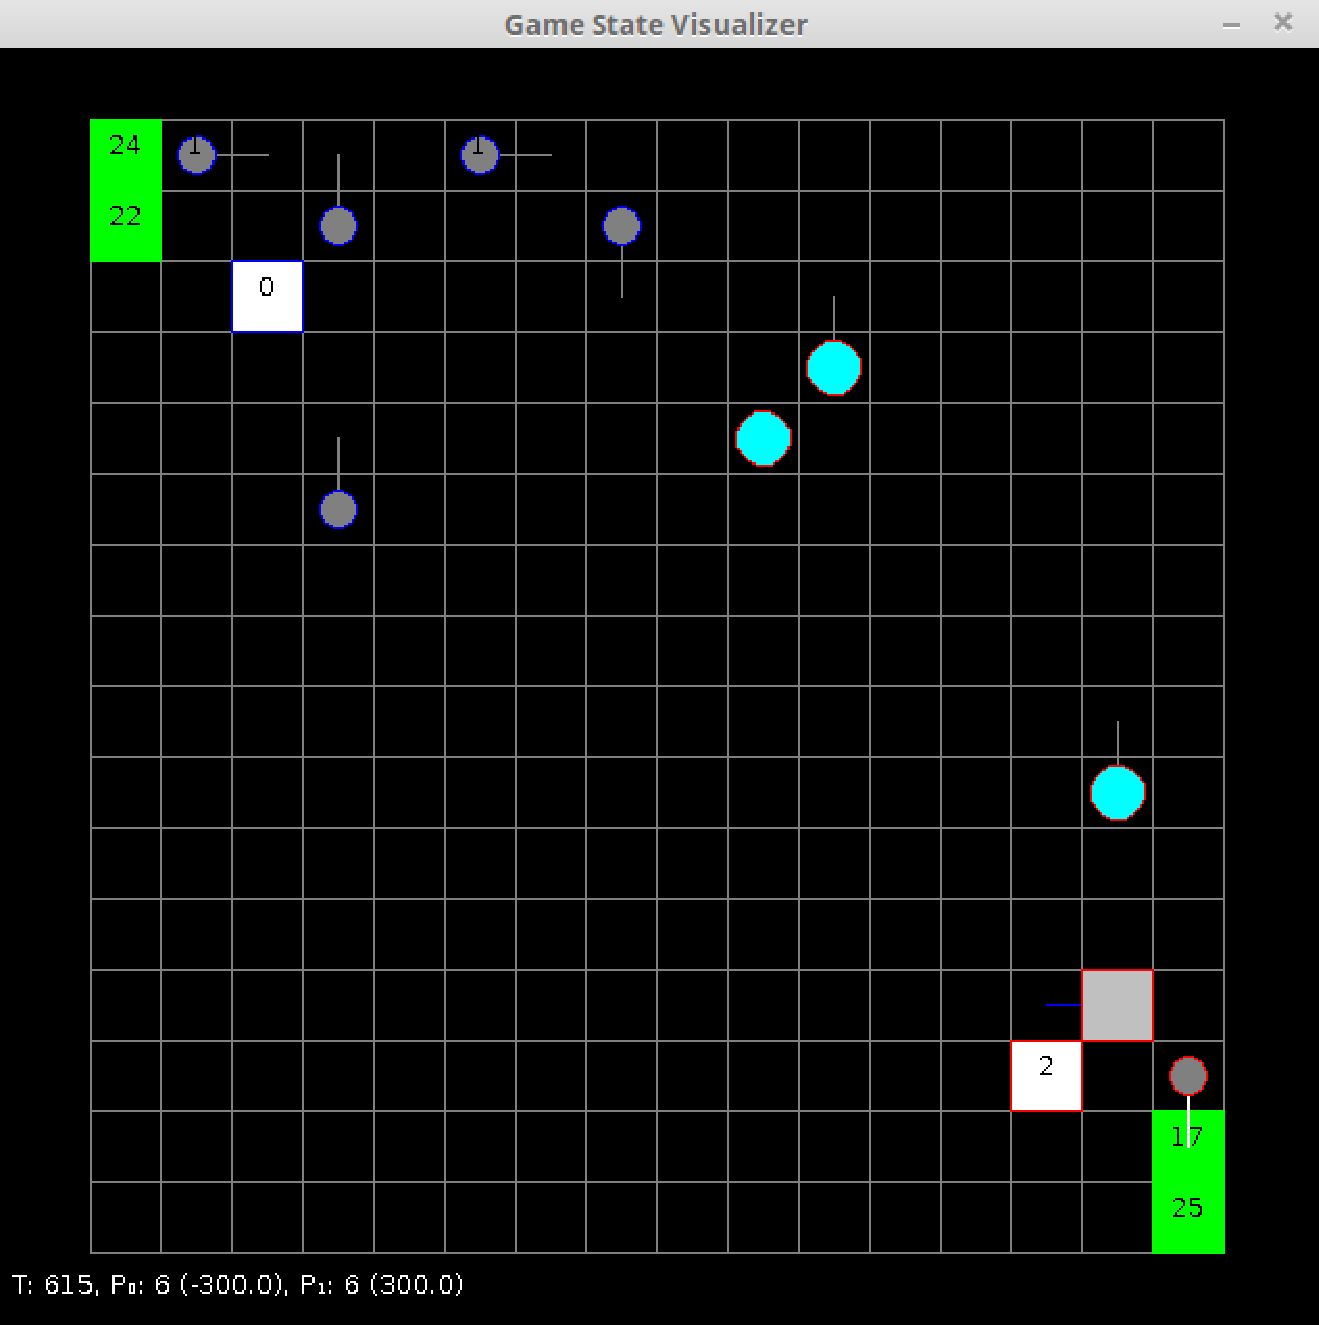
\includegraphics[width=0.5\linewidth]{fig/microRts.pdf}
		\captionof{figure}{Exemplo de tela do MicroRTS.}
		\label{fig:microrts}
	\end{center}	
	
	%---------------------------------------------------------------
	%	Implementação
	%---------------------------------------------------------------
	\color{NavyBlue}
	\section*{\huge Implementação}
	\color{Black}
	\begin{itemize}
		%[leftmargin=2em]\itemadjust
		\item A implementação do algoritmo foi feita na plataforma do MicroRTS, utilizando o SHOP2 para geração dos planos.
		\item Foram criados dois conhecimento de domínio pensando em cenários de jogo onde o jogador cria tropas para mandar destruir a base adversária.
		\item A primeira estratégia cria apenas uma unidade de ataque e manda atacar. Já a segunda estratégia enquanto está atacando também cria novas tropas.  
	\end{itemize}
	
	%---------------------------------------------------------------
	%	Experimentos e Resultados
	%---------------------------------------------------------------
	\color{NavyBlue}
	\section*{\huge Experimentos e resultados}
	\color{Black}
	
	\begin{itemize}
		%[leftmargin=2em]\itemadjust
		\item O MicroRTS possui técnicas de jogo implementadas para se jogar contra.
		\item As técnicas presentes no MicroRTS são usadas como adversário do algoritmo de AHTN. 
		\item Os experimentos foram executados em um mapa 16 por 16 e começando dos dois lados do jogo, o lado azul na parte superior, e o lado vermelho na parte inferior. Cada jogador inicia possuindo uma base, um trabalhador e dois recursos próximos a sua base.
		\item A Tabela~\ref{tab:resultados} ilustra os resultados obtidos.
	\end{itemize}
	
	\vspace{8mm}
	{\large
		\begin{center}
			\begin{tabular}{|c|cc|cc|}
				\hline
				\textbf{}           & \multicolumn{2}{c|}{\textbf{Lado Azul}}                    & \multicolumn{2}{c|}{\textbf{Lado Vermelho}}                \\ \hline
				\textbf{Adversário} & \multicolumn{1}{c|}{\textbf{Vitórias}} & \textbf{Derrotas} & \multicolumn{1}{c|}{\textbf{Vitórias}} & \textbf{Derrotas} \\ \hline
				\multicolumn{5}{|c|}{\textbf{Estrat\'egia 1}}                                                                                                   \\ \hline
				RandomAI              & 5                                      & 0                 & 5                                      & 0                 \\
				RangedRush              & 0                                      & 5                 & 5                                      & 0                 \\
				HeavyRush               & 0                                      & 5                 & 5                                      & 0                 \\
				LightRush               & 0                                      & 5                 & 5                                      & 0                 \\
				WorkerRush              & 0                                      & 5                 & 0                                      & 5                 \\ \hline
				\multicolumn{5}{|c|}{\textbf{Estrategia 2}}                                                                                                   \\ \hline
				RandomAI              & 5                                      & 0                 & 5                                      & 0                 \\
				RangedRush              & 5                                      & 0                 & 5                                      & 0                 \\
				HeavyRush               & 0                                      & 5                 & 5                                      & 0                 \\
				LightRush               & 0                                      & 5                 & 5                                      & 0                 \\
				WorkerRush              & 0                                      & 5                 & 0                                      & 5                 \\ \hline
			\end{tabular}
			\captionof{table}{Resultados do AHTN contra as técnicas do MicroRTS.}
			\label{tab:resultados}
		\end{center}
	}
	
	%---------------------------------------------------------------
	%	Referencias
	%---------------------------------------------------------------
	\large
	\color{NavyBlue}
	\section*{Referências}
	\renewcommand{\section}[2]{}
	\color{Black}
	\raggedright
	\bibliographystyle{plain}
	\bibliography{poster}
	
\end{multicols}
\end{document}